\documentclass[preprint]{acm_proc_article-sp}
\usepackage{graphicx}
\DeclareGraphicsExtensions{.jpg,.jpeg,.png}
\renewcommand{\baselinestretch}{1.0}
\begin{document}
\newcommand{\tmark}{^{\mbox{TM}}}
\title{GridPACK$\tmark$: A Framework for Developing Power Grid Simulations on High
Performance Computing Platforms}

\numberofauthors{11}
\author{
\alignauthor
Bruce Palmer\footnotemark[1]\\
\affaddr{bruce.palmer@pnnl.gov}
\alignauthor
William Perkins\footnotemark[1]\\
\affaddr{william.perkins@pnnl.gov}
\alignauthor
Yousu Chen\footnotemark[2]\\
\affaddr{yousu.chen@pnnl.gov}
\and
\alignauthor
Shuangshuang Jin\footnotemark[2]\\
\affaddr{shuangshuang.jin@pnnl.gov}
\alignauthor
David Callahan\footnotemark[3]\\
\affaddr{david.callahan@pnnl.gov}
\alignauthor
Kevin Glass\footnotemark[1]\\
\affaddr{kevin.glass@pnnl.gov}
\and
\alignauthor
Ruisheng Diao\footnotemark[1]\\
\affaddr{ruisheng.diao@pnnl.gov}
\alignauthor
Mark Rice\footnotemark[1]\\
\affaddr{mark.rice@pnnl.gov}
\alignauthor
Stephen Elbert\footnotemark[1]
\affaddr{stephen.elbert@pnnl.gov}
\and
\alignauthor
Mallikarjuna Vallem\footnotemark[1]\\
\affaddr{mallikarjun.vallem@pnnl.gov}
\alignauthor
Zhenyu (Henry) Huang\footnotemark[1]\\
\affaddr{zhenyu.huang@pnnl.gov}
\alignauthor
}

\toappear{\copyright 2014 Association for Computing Machinery. ACM
acknowledges that this contribution was authored or co-authored by an employee,
contractor or affiliate of the United States Government. As such, the United
States Government retains a nonexclusive, royalty-free right to publish or
reproduce this article, or to allow others to do so, for Government purposes
only.}

\maketitle
\begin{abstract}
This paper describes the GridPACK\texttrademark framework, which is designed to help
power grid engineers develop modeling software capable of running on high
performance computers. The framework makes extensive use of software templates to
provide high level functionality while at the same time allowing developers the
freedom to express whatever models and algorithms they are using.
GridPACK\texttrademark contains modules for setting up distributed
power grid networks, assigning buses and branches with arbitrary behaviors to
the network, creating distributed matrices and vectors and using parallel linear
and non-linear solvers to solve algebraic equations. It also provides mappers
to create matrices and vectors based on properties of the network and
functionality to support IO and to manage errors. The goal of
GridPACK\texttrademark is to substantially reduce the complexity of
writing software for parallel computers while still providing efficient and 
scalable software solutions. The use of GridPACK\texttrademark is illustrated
for a simple powerflow example and performance results for powerflow and dynamic
simulation are discussed.
\end{abstract}

\keywords{Electric Power Grid, High Performance Computing, Software Frameworks}

\renewcommand{\thefootnote}{\fnsymbol{footnote}}
\footnotetext[1]{Pacific Northwest National Laboratory, Richland, WA, 99352}
\footnotetext[2]{Pacific Northwest National Laboratory, Seattle, WA}
\footnotetext[3]{Northwest Institute for Advanced Computing, Seattle, WA}

\section{Introduction}
The electric power grid has been characterized as being the largest machine in
the world, but in spite of this it is still being modeled primarily on workstations running
serial programs. Much smaller systems (e.g. the internal combustion
engine\cite{EXACT}) are, on the other hand,
being modeled in ways that can fully exhaust the resources of
the largest available computing systems. Power grid engineers have spent
enormous effort and ingenuity reducing simulations of the grid to manageable sizes,
but these reductions have resulted in approximations and loss of detail which may
be hiding or obscuring important features and behaviors of the electric power
grid.
Furthermore, as more energy is derived from renewable sources, the
complexity and unpredictability of the grid will increase. The influx of more
information from data sources such as smart meters is also making the task of modeling
even small networks more challenging. The power grid is clearly an
appealing target for high performance computing (HPC) but few
tools are available to assist power grid engineers interested in writing code
that runs on HPC platforms.

Existing power grid modeling tools that are widely used by today's utilities are
built on serial kernels, some of which represents legacy code going back decades.
These
codes used array-based models of programming, in spite of the heterogeneity of
power grid networks. In many cases, codes have not made use of modern,
object-oriented constructs, even though these
would be a natural fit. Furthermore, most of the code used in power grid
modeling is proprietary commercial software, so there is no access to the source
code and development is not focused on creating modules that can be used in a
general context. Even when access to the source code is available, it still
requires significant code redesign and reconstruction to utilize HPC
technologies, partly because these serial codes have been highly optimized to
run on single processors. Some recent efforts have been to made to construct
parallel versions of power grid simulations, but these have been single
application development efforts and again, have not resulted in software that is
useful across multiple applications. Recent examples of parallel power grid
applications include power flow\cite{LUO}, contingency
analysis\cite{HUANG,CHEN}, state estimatio\cite{FALCAO,CHEN} and dynamic
simulation\cite{JIN}.

This paper will describe the GridPACK\texttrademark framework for developing parallel
power grid simulations that run on HPC platforms with high levels of
performance and scalability. Frameworks have appeared in other contexts and been
used to reduce the programming burden on domain scientists by making complex
but commonly used motifs available through libraries or other mechanisms.
Both the Community Climate System Model\cite{CCSM} and Weather Research
and Forecasting Model\cite{WRF} are framework-based
approaches to developing climate and weather models. The Cactus framework is
designed to support grid-based applications and is widely used in the numerical
general relativity community\cite{CACTUS}. The Common Component
Architecture\cite{CCA} is a framework
designed to support modularization of codes and has been used successfully in
some groundwater applications\cite{SPH}. Other examples of frameworks or modular approaches
to code development can be found, particularly among large software projects
with a broad developer base.

The GridPACK\texttrademark framework is designed to allow power
system engineers to focus on developing working applications from their
models without getting bogged down in the details of decomposing the computation
across multiple processors, managing data transfers between processors, working out
index transformations between power grid networks and the matrices generated by
different power applications, and managing input and output. The framework
relies heavily on software templates to allow users to develop
application-specific components that can then be plugged into generic modules
that handle many of the more complicated book-keeping tasks. The description of
network components and their contributions to algebraic equations are left to
the application developer, but many other functions can be handled by the
framework itself. These include creating distributed
network objects, setting up distributed matrices and vectors, linear and
non-linear solvers and IO. This approach provides
flexibility where it is needed, in the specification of the models and equations
that are to be addressed by the application, while encapsulating much of the
tedious book-keeping and index calculations associated with programming in a
distributed environment.
The following will summarize the overall design of the GridPACK\texttrademark
framework and then describe the major modules and some applications that have
been developed with them.

\section{GridPACK\texttrademark Software Stack}
GridPACK\texttrademark is currently available as a collection of C++ modules and
has taken a strongly object-oriented approach to software development. Power
grids can be thought of as directed graphs with nodes (referred to as buses in
power grid terminology) representing elements such as generators, loads, etc.
and edges (branches in power grid terminology) representing transmission lines
and  transformers. The core software objects are user-developed descriptions of
the properties and behavior of buses and branches. Bus and branch objects
specify all the properties of the power grid and are also responsible for
evaluating the contribution of the network element to whatever equations are
going to be used in the power grid analysis.

The network components are derived from base classes that specify a set
of virtual functions that can be implemented by the user. Depending on the
application, some or all of these functions can be implemented. Those that are
not implemented default to simple no-ops. In addition, a few functions are
provided that are used either internally by other parts of the framework or are
intended for use by developers as is. These include operations such as obtaining
a list of objects that are connected to the requesting object and returning the
unique integer identifier of a bus.

The user-developed base and branch components can then be embedded in the rest
of the framework and used to create different power grid applications. A
schematic picture of the framework software stack is shown in Figure
\ref{schematic}.
\begin{figure}
\centering
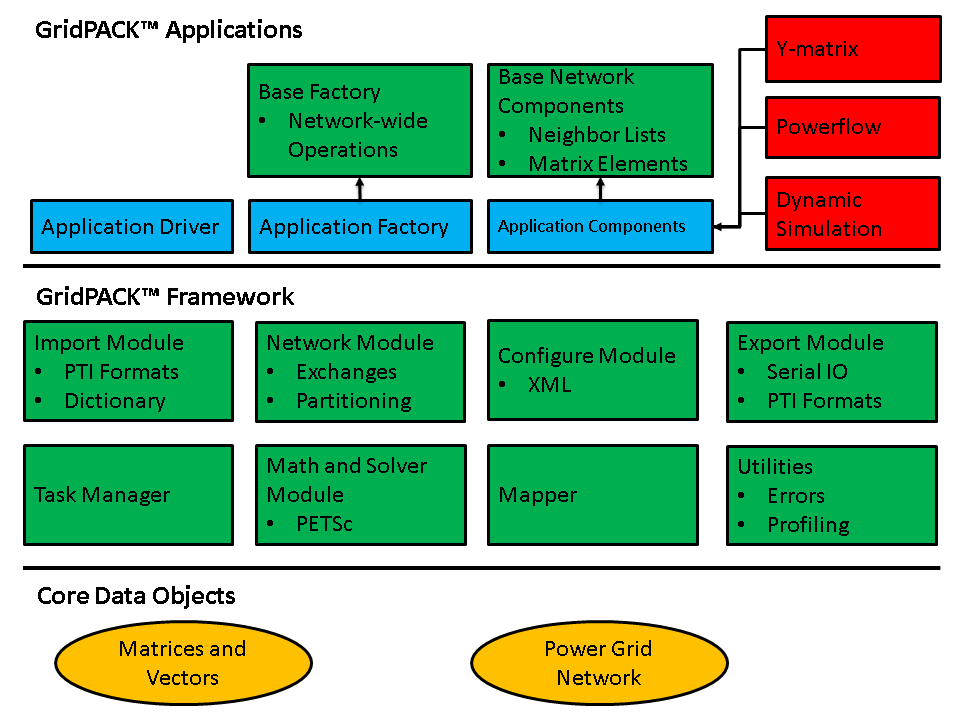
\includegraphics[width=3.5in,keepaspectratio=true]{./Fig1}
\caption{\label{schematic} A schematic diagram of the GridPACK\texttrademark
software stack. Framework modules are colored green, user-supplied modules are
colored blue. User modules that can be used across multiple applications are
colored red.
}
\end{figure}
The core data objects in most power grid applications are a representation of
the power grid network and matrices and vectors that are generated by the
equations describing the system. A key requirement of a power grid-oriented
framework is to provide distributed representations of these objects.
GridPACK\texttrademark contains modules for creating both distributed networks
and distributed algebraic objects. In addition, GridPACK\texttrademark also
supplies a set of components that can be used to map between the two.

Many of the modules in GridPACK are software templates and can be used to create
application-specific instances. The network class is a template that depends
on user-supplied bus and branch classes. Other modules in the framework depend
on the network, so once the buses and branch classes are specified, they can be
used to create application-specific versions of many of the remaining modules.

In addition to the bus and branch class, the application developer is
responsible for generating two other classes. The first is a factory that
is responsible for operations that run over the entire network
and the second is a high
level application driver that controls overall program flow and implements the
solution algorithm. The user factory inherits from a base factory class that
contains some important initialization functions. Additional functions usually
consist of operations that
trigger a method on each bus and branch. The application driver instantiates the
network, reads in a network configuration from an external file and runs the
partitioning algorithm on it, creates the mappers that can be used to generate
the matrices and vectors used in the algebraic equations that are to be solved as
part of the analysis, implements the solution algorithm and writes the results
to output. The actual driver code itself is fairly compact and consists
primarily of calls to other modules.

A diagram showing the relationship of the basic software classes to each other
is shown in Figure \ref{templates}.
\begin{figure}
\centering
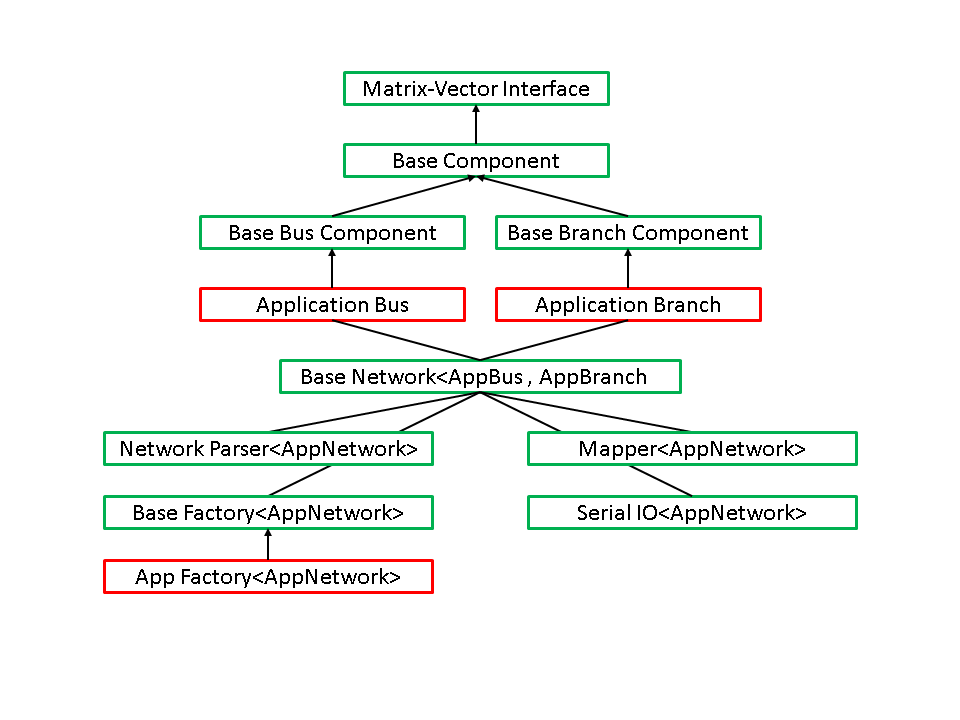
\includegraphics[width=3.5in,keepaspectratio=true]{./Fig2}
\caption{\label{templates} A schematic diagram illustrating the relationship of
different GridPACK\texttrademark software classes to each other.
Framework classes are colored green and user-supplied supplied classes are
colored blue. }
\end{figure}
The application developer is responsible for creating the application bus
and branch classes, most of the application-specific behavior of the framework
is then derived from the application buses and branches. The factory
class can also be customized to support network-wide operations that are
specific to a particular application. The only remaining code that requires
user development is the driver which controls the overall behavior
of the application. As discussed below, this can be written at a high
level and is relatively compact.

GridPACK targets three major functionalities
\begin{itemize}
\item Distributed graphs representing the topology of the power grid
\item Distributed matrices and vectors and parallel solvers and
preconditioners. The solution algorithms for power grid problems are usually
expressed in terms of linear or non-linear algebraic equations. 
\item The mapping of objects located on the network to distributed matrices and vectors.
For example, the diagonal elements of the admittance matrix are associated with
buses and the off-diagonal elements are associated with branches. The mapping
between the network and matrix elements can be automated to a considerable
extent.
\end{itemize}
Additional functionality provided by the framework supports IO, task management,
profiling, error handling, etc. 

The network class manages distribution of the power grid, partitioning of the
network and exchange of ghost data between processors. Ghost buses and branches
represent copies of network components that are owned by other processors but
are directly connected to elements on the local process. In order to update
the state of local objects, it is often necessary to have current values for
ghost components and this requires interprocessor communication.

The network also serves as a container for the objects that define the behavior
of buses and branches in the actual power grid model. Bus and branch behaviors frequently
depend on the objects immediately attached to them so that buses depend on the
branches that are attached to them (and possibly on the buses attached to them
via a branch) and branches depend on the buses attached at either end of the
branch. Providing easy access to these attached objects is another function of the
network module.

Basic algebraic objects, such as matrices and vectors, are a core part
of the solution algorithms required by power grid analyses. These also tend to
be large data objects that must be distributed across processors. Furthermore,
the solution algorithms built around these data objects are generally the most
time-consuming part of program execution, so it is necessary to ensure that the
solutions are fully parallel as well. Most solution algorithms
are dominated by sparse matrices but a few, such as Kalman filter
analyses\cite{KAL} and dynamic simulation\cite{DS}, require dense
matrices. Vectors are typically dense. There exists a rich set of libraries for
constructing distributed matrices and vectors and these also contain preconditioner
and solver capabilities.  GridPACK\texttrademark leverages this work heavily by
creating wrappers around these libraries that can be used in solution
algorithms. Wrapping these libraries instead of using them directly has the
advantage that creating these algebraic objects can be simplified somewhat for power grid
applications but more importantly, it allows developers to investigate new
solver and algebraic libraries seamlessly, without disrupting other parts of the code.
The current GridPACK\texttrademark implementation is built on top of the
PETSc\cite{PETSC}
libraries but other possibilities include Hypre\cite{HYPRE} and
Trilinos\cite{TRIL}. All these
libraries support distributed matrices and vectors, basic algebraic operations
such as matrix-vector multiply, inner products, etc. and a variety of solution
methods for linear and non-linear equations.

Finally, there is a need to support the generation of matrices from objects in the
network and the ability to push data from solution vectors back down into
network objects. This is one of the most complicated and error-prone parts of
writing code, especially for parallel platforms. Much of the work involved in
setting up matrices can be eliminated by having users implement a few functions
that provide the individual matrix elements contributed by each bus or branch. The
mapping function can then assemble these elements into a complete matrix for the
entire system. The fact that developers can focus on writing code for individual
matrix elements reduces the amount of programming required and fits in more
intuitively with the physical models. The complicated index calculations
required to evaluate global offsets that are needed to set up a distributed
matrix can be left to the framework.

These three capabilities are at the core of GridPACK\texttrademark, but numerous
additional modules are built around them. These include import modules for injesting
network configuration files and using these to set up a network object, output
modules that can be used to gather data from buses and branches and write them
to output, a task manager that can be used to partition tasks out to either separate
processors or to processor groups to support multiple levels of parallelism, a
configuration module to manage input from an XML-based input deck, profiling and
error handling. Many of these are also templated from the network class  and
some can be customized to particular networks by modifying methods in the bus
and branch classes.

As already mentioned, GridPACK\texttrademark is written in C++, although work
on a Fortran interface is currently in progress. Communication is handled
through a combination of the Message Passing Interface (MPI)\cite{MPI1} and
Global Arrays\\
(GA)\cite{GA} communication libraries. The matrix and solver
functionality comes from the PETSc\cite{PETSC} libraries and network partitioning
is accomplished using Parmetis\cite{PARMETIS}.

\section{GridPACK\texttrademark Mappers}
The network module is responsible for distributing the network across available
processors. Figure \ref{wecc} shows a partition of the Western Electric
Coordinating Council (WECC) network across 16 processors. This partition results
in each processor containing a relatively connected subnetwork with minimal
connections to other processors. Once the network is partitioned, the
problem of mapping matrix elements generated from the buses and branches becomes
a formidable challenge. This is further complicated by the fact that for many
applications, not all buses and branches contribute the same number of elements
and some may contribute nothing at all. Assigning global indices to these
elements in a consistent way that also matches the row-block partition of the
distributed matrices can be a daunting challenge, even for experienced parallel
programmers.
\begin{figure}
\centering
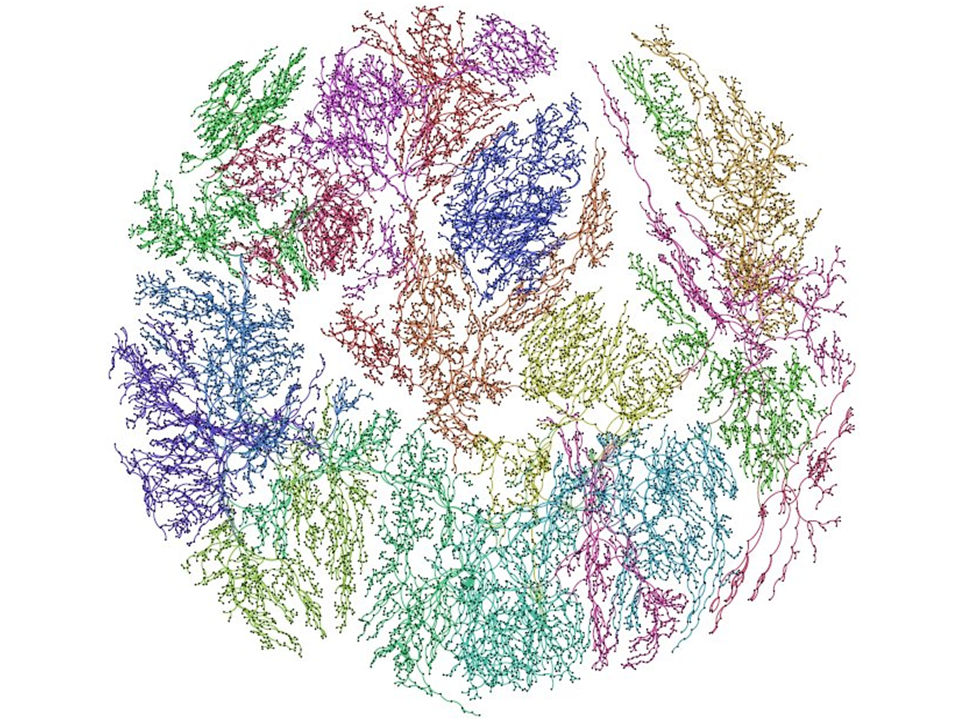
\includegraphics[width=3.5in,keepaspectratio=true]{./Fig3}
\caption{\label{wecc} Partitioning of the WECC network across 16 processors. Each
color represent the buses and branches associated with a different processor.
}
\end{figure}

The mapper module is designed to simplify this process considerably. It works in
conjunction with routines defined in the base component classes that
require each bus and branch to provide a list of matrix elements contributed by
that network component. For many grid applications, such as power flow and dynamic
simulation, both the dependent and independent variables are associated with
the buses so buses are associated with diagonal blocks and branches with
off-diagonal blocks. The functions in the base network component class
return the dimension of the matrix block associated with that component and the
values of the matrix elements. For most applications, these blocks are
relatively small, on the order of $1\times 1$ or $2\times 2$ for diagonal
blocks. Furthermore, the values of the matrix elements contributed by any
network component only depend on properties of components that are immediately
connected to that component. For example, a diagonal element $Y_{ii}$ of the
Y-matrix, which is used in a great many power grid applications,
can be written as a sum
\[
Y_{ii} = -\sum_j Y_{ij}
\]
The diagonal element $Y_{ii}$ is evaluated on bus $i$ and the terms $Y_{ij}$
exist on the branches connected to bus $i$. The evaluation of the matrix element
is relatively local and can be performed by looping over connected elements.

The way the mapper uses these elements is illustrated in Figure
\ref{mapper}. Figure \ref{mapper}(a) shows a hypothetical network.
Figure \ref{mapper}(b) shows the contributions to the matrix from all buses
and branches. Note that some network components contribute nothing, and
not all components contribute the same sized blocks.  The mapping of the individual
block from the network in Figure \ref{mapper}(b) to initial matrix locations
based on network location is shown in Figure \ref{mapper}(c). This is followed
in Figure \ref{mapper}(d) by the elimination of gaps in the matrix due to rows
and columns with no values.
\begin{figure}
\centering
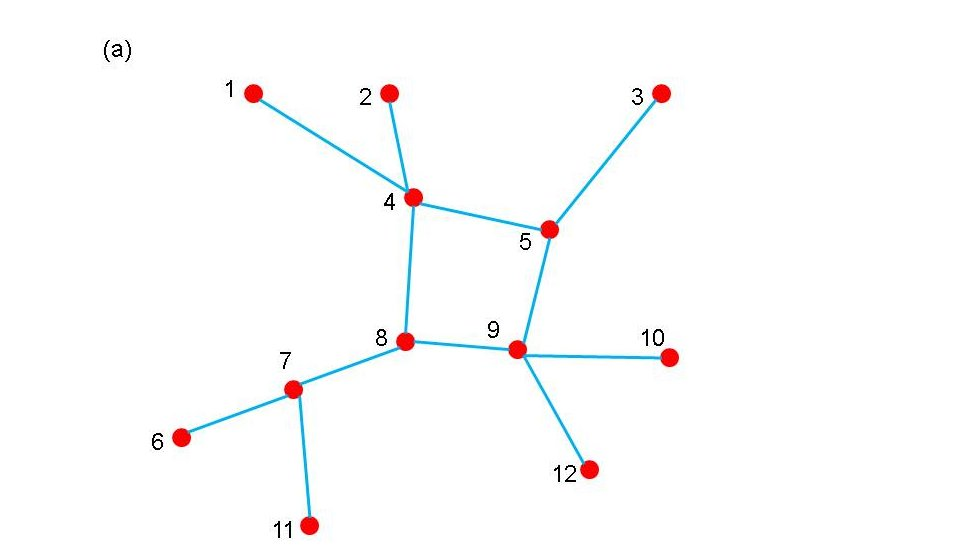
\includegraphics[width=3.5in,keepaspectratio=true]{./Fig4a}
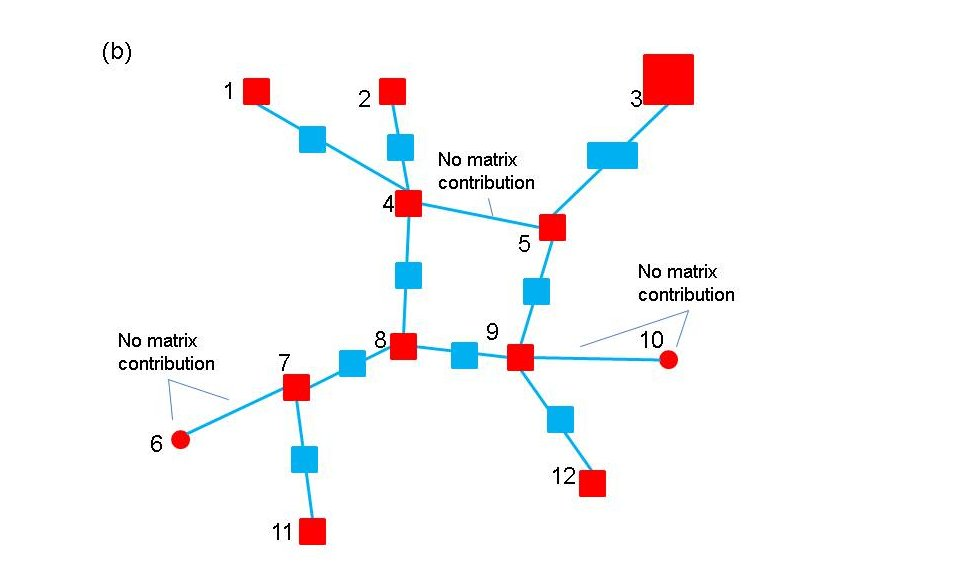
\includegraphics[width=3.5in,keepaspectratio=true]{./Fig4b}
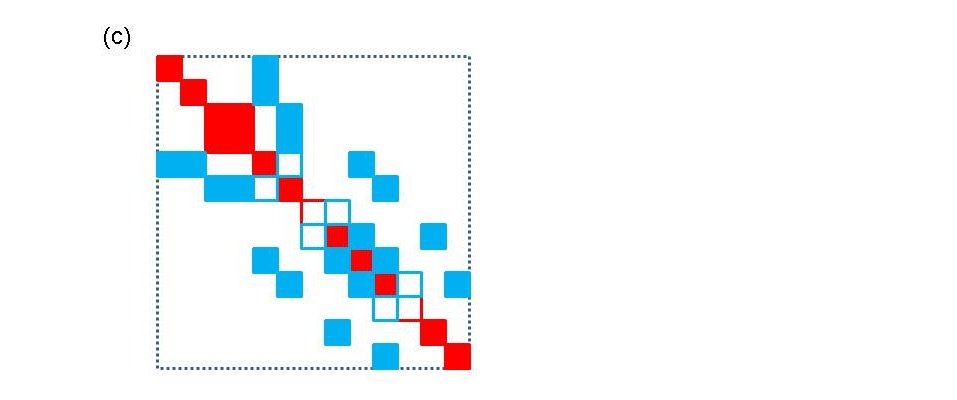
\includegraphics[width=3.5in,keepaspectratio=true]{./Fig4c}
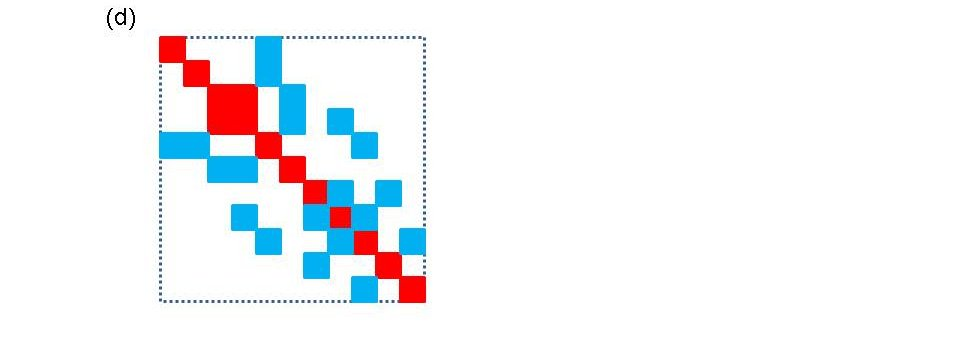
\includegraphics[width=3.5in,keepaspectratio=true]{./Fig4d}
\caption{\label{mapper} A schematic diagram of the matrix map function.
(a) a small network (b)
matrix blocks associated with branches and buses. Note that not all blocks are
the same size and not all buses and branches contribute (c) initial construction
of matrix based on network indices (d) final matrix after eliminating gaps
The bus numbers in (a) and (b) map to approximate column locations in (c).}
\end{figure}

An example of a matrix generated using the GridPACK\texttrademark\\
mappers is
shown in Figure \ref{matrix}. The matrix is distributed on 4 processors.
\begin{figure}
\centering
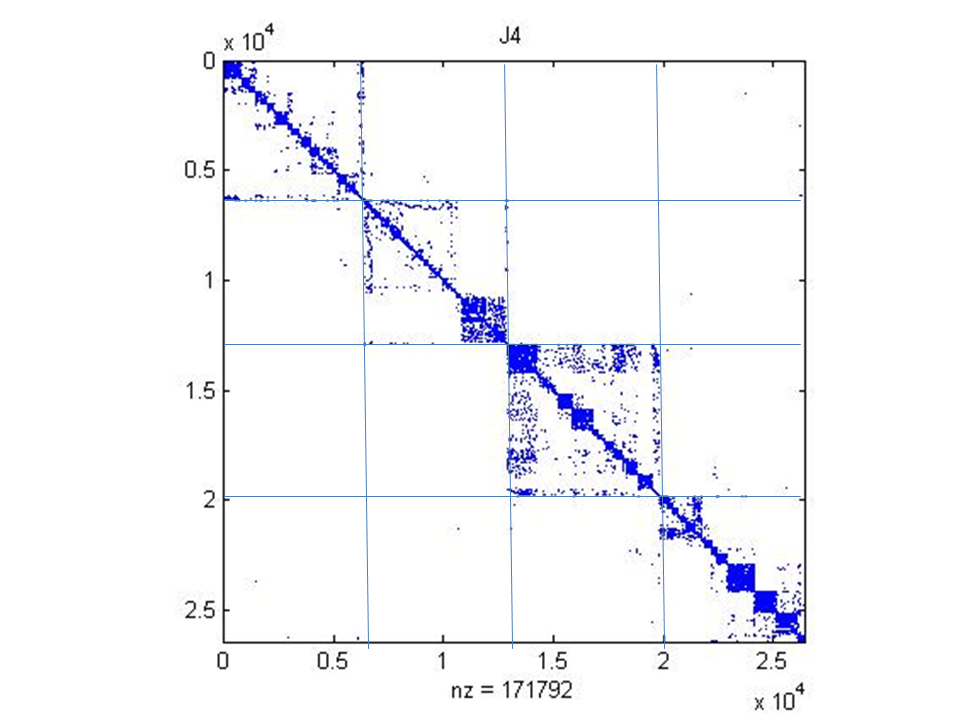
\includegraphics[width=3.5in,keepaspectratio=true]{./Fig5}
\caption{\label{matrix} Fill pattern for the Jacobian matrix for a power flow
calculation on the WECC network on 4 processors. The lines are a guide to the
eye. The 4 blocks on the diagonal
represent connections between buses on the same processor, the remaining elements
are between buses on different processors}
\end{figure}
The large blocks along the diagonal represent connections between buses on
the same processor, matrix elements outside these blocks are generated from
branches connecting buses on different processors. The block structure is the
result of creating internal indices such that all the buses that are owned by
a processor are indexed consecutively. The block structure should also improve
the performance of preconditioners used with the solvers.

A more general matrix-vector interface has been developed that can handle systems
where
dependent and independent variables are associated with both buses and branches.
This occurs in applications such as state estimation\cite{SE}, Kalman filter
analysis and
market optimization. However, the generalized interface and the associated
mappers still only need local information in order to implement the functions in
the interface that are used to build matrices. These remain relatively simple
calculations and do not require complex index evaluations on the part of
application developers.

\section{Math Library Interface}
The math module in
GridPACK\texttrademark relies on the PETSc libraries for its solvers and support
for distributed matrices and vectors.
The current math interface supports the creation of both sparse and dense
distributed matrices and distributed vectors and provides access to a broad
spectrum of linear and non-linear solvers. Different solvers can be accessed by
using PETSc's runtime options data base, which can invoke different solvers using
string arguments. These strings can be extracted from the input deck and passed
through to the math module using the configuration module.

In addition to constructing matrices and vectors, the math interface supplies
many basic algebraic operations. These include various types of norms ($L_2$,
$L_{\infty}$, etc.), matrix-vector multiplies, matrix transpose, scaling by a
value, addition, etc. Linear and non-linear solvers are also supplied by the
interface. The solver interfaces are relatively simple and most functionality
is accessed by
specifying options in the input deck that are passed directly to the solver.
Alternatively, the interface could support different solvers and these would be
accessed by instantiating different solver objects at the application level
based on user input. However, this leads to a more complicated interface with
likely dependencies on the underlying math library. A smaller interface that
relies on runtime options is more transferable between different libraries,
although it is likely that the user input file would have to change if an
application was linked to a different math module implementation.

\section{Communication in GridPACK\texttrademark}
GridPACK\texttrademark relies on both MPI\cite{MPI1} and Global Arrays\cite{GA}
for communications.
To support multiple levels of parallelism and multiple-task algorithms, it was
important to guarantee that GridPACK could run on process groups beyond the
world group. This meant creating a GridPACK\texttrademark\\
communicator class
that contained both an MPI communicator and a GA processor group. The network
class is instantiated with a communicator and this can be used to restrict the
network to a subset of processors. This behavior then passes down to any
objects that are instantiated from the network. Networks distributed over a
subset of processors are needed for applications such as contingency
analysis\cite{CA}
that run many independent parallel tasks.

Many of the other modules in GridPACK\texttrademark use GA for communication.
The primary reason is the availability of the GA gather, scatter and
scatter-accumulate calls. These functions allow random access to individual
elements in a distributed array of data. The GA gather/scatter functions are
one-sided and can be called from any process without a
corresponding call on another process. Data consistency must be maintained by
the programmer using global synchronization calls that consist of a combination
of a fence, to flush out all outstanding communication, and a barrier.

The gather and scatter calls can be used to implement functions such as the ghost
bus and ghost branch updates in a straightforward array. For example, each of
the buses that is local to a process is given an internal index such that all
the local buses on a process are indexed using a consecutive set of integers and
the overall set of integers runs from 0 to $N-1$, where $N$ is the total number
of integers. A one-dimensional distributed GA array is created such that the
portion of the array that is local to each process is the same size as the
number of local buses. The size of the individual data elements is equal to the
size of the total amount of data that each bus must exchange in a ghost bus update
operation. Note that although different buses may behave in different ways, with
some functionality turned on or off, the amount of data exchanged must reflect
the total amount of data that {\em could} be needed on a remote bus. This has to
be done because all data elements in a GA array must be the same size.

In the first stage of the update, the information from all local buses is
scattered to the global array. This operation is fast because all data transfers
are on the same process and only involve shared-memory copies. A synchronization
operation is then implemented to flush out all outstanding communication
and thereby guarantee that the GA is in a known state. Failing to implement a
synchronization can result in a race condition that can cause some buses to
receive stale data. Each process can then copy the
data elements to its ghost buses using a GA gather call. The entire process is
illustrated schematically in Figure \ref{update}.
\begin{figure}
\centering
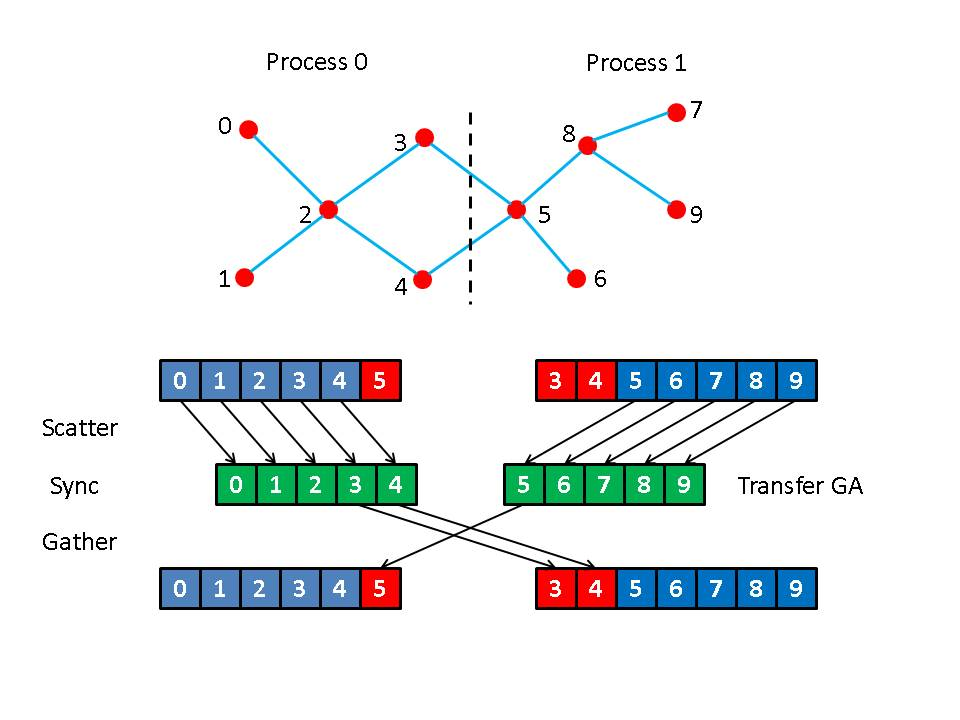
\includegraphics[width=3.5in,keepaspectratio=true]{./FigU}
\caption{\label{update} Schematic diagram of network bus update operation for a
small network distributed on two processors. The local arrays of buses are
denoted by the blue and red boxes, the global array used for transferring data
is represented by the green boxes
}
\end{figure}

The one-sided gather-scatter functionality is also used 
to implement the mappers. The construction of the matrices from network
contributions requires a calculation to determine what the offsets in the
target matrix are for the rows and columns associated with each of the locally
owned buses. This information needs to be made globally available so that the
off-diagonal contributions to the matrix, which come from the branches, can be
properly placed in the matrix as well. The one-side gather-scatter operations,
as well one-sided get and put operations (which move blocks of data) are used to
implement these calculations.

% Another class of operations needed in many power grid applications are
% mechanisms for moving input data associated with buses and branches to the
% processors that own those buses and branches. This is more difficult than it
% might initially seem. Network buses are typically indexed by a unique positive
% integer but there is no requirement that the integers be consecutive or run from
% 1 to $N$. Branches are indexed by the pair of buses at either end. Mapping data
% coming into the calculation from a source other than the file that contains the
% network configuration itself can be a complicated problem. If the number of data
% elements is small, then the entire list can be broadcast to all processors and
% each process can select those elements that apply to buses and/or branches that
% are locally held. However, if the list of data elements is large, such as in a
% state estimation calculation, then this could potentially create a memory
% bottleneck.

% To provide a mechanism to directly map data from the original indices to the bus
% and branch objects that need it, GridPACK\texttrademark has implemented a
% distributed hash
% functionality. For power grid applications, the requests to the hash table can be
% made into collective operations, which considerably simplifies implementation.
% As an example, we will consider the mapping of the network bus
% indices and branch index pairs to internal global indices that have the
% desirable property of runing from 0 to $N-1$ for buses and 0 to $M-1$ for
% branches ($M$ is total number of branches). This can be accomplished by 1)
% creating a hash function that maps each original bus index or branch index pair
% to a processor 2) Use the hash function to create a linked list of the data
% going to each processor 3) use an MPI Alltoall call to determine how much data
% is going to be received from each processor 4) based on the information from the
% Alltoall call set up buffers to receive index pairs and exchange these using an
% Alltoallv call 5) store the index pairs in a local hash table. The map between
% the original index and the global index can be recovered using a  second collective
% call. In this case, a list of original indices or index pairs is given as input
% and the corresponding list of global indices is given as output. The
% implementation is similar to the distributed hash table construction 1) a linked
% list of original indices is created using the hash function 2) the requested
% values are sent to the process that owns them using Alltoall and Alltoallv calls
% 3) each process uses its local hash table to match the original indices with the
% global index 4) the global indices can be sent back to the process that
% requested them with a single Alltoallv call. The distributed hash functionality is
% general and other index pairs can be created with it. If necessary, something
% besides indices or index pairs could be used as the keys, but this has not
% proved necessary so far. By setting up the hash table and accessing data using
% collective calls, we have eliminated the need for an independent process running
% on a remote processor that manages hash requests.

\section{Programming Applications with GridPACK\texttrademark}
The top-level driver for a GridPACK\texttrademark is relatively simple and
comparable in complexity to scripting languages such as Python or Matlab. An
example driver for a power flow application (one of the basic power grid
calculations) is shown in Figure \ref{code}. Before discussing this code, it
should be noted that the bulk of the effort in creating the power grid application
was in writing the bus and branch classes (in this case the PFBus and PFBranch
classes). However, these classes are also the most reusable. For example, many
power grid applications, including this one, require the calculation of a
Y-matrix, or at least need to use its matrix elements as parameters in other
calculations. Thus, a good implementation of the Y-matrix bus and branch classes
can be used across many applications by inheriting from them to create
bus and branch classes for more specific uses. This promotes software reuse and
also makes it possible to propagate improvements or bug fixes to the Y-matrix
classes easily to other applications that use it. In Figure \ref{schematic}, the
bus and branch classes represented by the boxes in red have all been used in
more than one application.

The power flow driver shown in Figure \ref{code} does not have many of the
features that an actual application would have, including the ability to set
parameters
from an external input file, output of results and profiling of timing behavior,
but it is sufficient to implement an actual powerflow calculation using
a Newton-Raphson iterative loop to get a solution for the non-linear power flow
equations. The driver starts by defining the power
flow network and factory classes (lines 1 and 2). It then creates a communicator
for the entire world group of processors and uses it to create a network
instance (line 4). The application then creates a network configuration parser
for configuration files using the PSSE/version 23 format and uses this to injest
a configuration from the file ``network.raw'' (lines 7 and 8). The network is then
distributed across processors in a form suitable for calculation by calling the
network method ``partition'' (line 9). At this point, the network is distributed
across processors and the buses and branches have been created. The parameters for each
bus and branch from the network configuration file are stored in a generic data
collection object.

In lines 11 through 14 a factory object is created and used to finish
initializing the network. The factory load method calls a load method in the
network component base class that takes the data collection object on each bus
and branch as an argument. The component level load method extracts the contents
of the data collection object and uses these to initialize the corresponding bus
or branch. After calling the load method, the buses now have all their
properties and behaviors set and can be used in computation.
The setComponents method initializes internal
indices that are used in the mappers It also sets a list of pointers in the
buses that point to all the neighbor branch and two pointers in the branches
that point to buses at each end of the branch. This enables the buses and
branches to access attached elements directly without having to go through the
network object. The setExchange sets up the internal exchange buffers that allow
ghost components to be updated with current information from remote processors.

The initBusUpdate initializes data structures that are used in data exchanges
between processors. This calculation does not need to update information on
ghost branches so there is no corresponding call to initialize a branch update.
The calls to the factory methods setYBus and setSBus loop over network
components and call a corrsponding method each of the buses and branches. These
perform internal calculations to evaluate the matrix elements of the Y-matrix
and some values that are used to set up the right hand side vector in the
powerflow calculation. Line 20 sets the mode to RHS. This causes an internal
parameter in all the buses and branches to be set to the value RHS and controls
what set of values are returned by the matrix-vector interface when a matrix
mapper is instantiated (line 21). In line 22, the mapper is used to create a new
distributed vector PQ that represents the right hand side of the powerflow
equations. Line 24 is used to switch the mode to Jacobian. Line 25 creates a
mapper that is used to create the Jacobian matrix in the powerflow equations and
line 26 creates the first iteration of this matrix. Line 27 makes a copy of the
right hand side vector that can be used for the solution.

Lines 29 through 33 set some control parameters and create a linear solver
instance. Line 37 then solves the equations for the current values of J and PQ
and returns the solution in X. The $L_{\infty}$ norm is evaluated in line 38 and
used
to set the initial value of the tolerance variable. If this is less than the
tolerance threshold, then the calculation is done, otherwise it enters the
iterative Newton-Raphson loop. This is similar to the calculation of the first
solution, with the exception of the call to mapToBus at line 43 and the network
updateBuses at line 44. The mapToBus call pushes the values from the solution back
into the network buses and updates internal bus parameters. The updateBuses call
distributes these updated values to the ghost buses. The calculation then
recalculates the Jacobian and right hand side vector and produces a new
solution. This continues until either the convergence threshold is reached or
the iteration count is exceeded.

The main feature of the code is that the solution algorithm is expressed at a
fairly high level and involves abstractions representing matrices and vectors
and the network. It does not require any of the internal details of these
objects, so the algorithm can be written in a compact manner. Other algorithms
involving the same algebraic objects could also be explored easily with minimal
code development.

\begin{figure}
\label{code}
\begin{verbatim}
 1  typedef BaseNetwork<PFBus,PFBranch> PFNetwork;
 2  typedef BaseFactory<PFNetwork> PFFactory;
 3  Communicator world;
 4  shared_ptr<PFNetwork>
 5      network(new PFNetwork(world));
 6
 7  PTI23_parser<PFNetwork> parser(network);
 8  parser.parse("network.raw");
 9  network->partition();
10
11  PFFactory factory(network);
12  factory.load();
13  factory.setComponents();
14  factory.setExchange();
15
16  network->initBusUpdate();
17  factory.setYBus();
18
19  factory.setSBus();
20  factory.setMode(RHS); 
21  BusVectorMap<PFNetwork> vMap(network);
22  shared_ptr<Vector> PQ = vMap.mapToVector();
23
24  factory.setMode(Jacobian);
25  FullMatrixMap<PFNetwork> jMap(network);
26  shared_ptr<Matrix> J = jMap.mapToMatrix();
27  shared_ptr<Vector> X(PQ->clone());
28
29  double tolerance = 1.0e-6;
30  int max_iteration = 100;
31  ComplexType tol;
32  LinearSolver solver(*J);
33
34  int iter = 0;
35
36  // Solve matrix equation J*X = PQ
37  solver.solve(*PQ, *X);
38  tol = PQ->normInfinity();
39
40  while (real(tol) > tolerance &&
41         iter < max_iteration) {
42    factory.setMode(RHS);
43    vMap.mapToBus(X);
44    network->updateBuses();
45    vMap.mapToVector(PQ);
46    factory.setMode(Jacobian);
47    jMap.mapToMatrix(J);
48    solver.solve(*PQ, *X);
49    tol = PQ->normInfinity();
50    iter++;
51  }
\end{verbatim}
\caption{\label{pf_app}. Top-level driver for a powerflow application using
GridPACK\texttrademark.}
\end{figure}

The results of a scaling study on the power flow code implemented using
GridPACK\texttrademark are shown in Figure \ref{powerflow} for an
artificial power grid network consisting of 777646 buses.
\begin{figure}
\centering
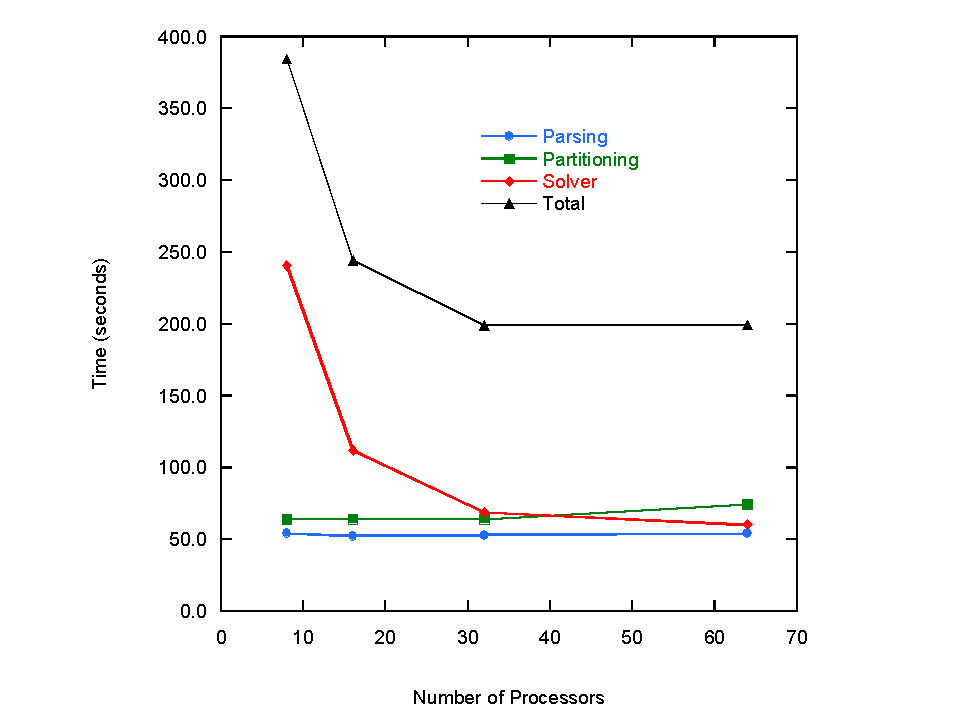
\includegraphics[width=3.5in,keepaspectratio=true]{./Fig8}
\caption{\label{powerflow} Strong scaling results for a powerflow calculation
using on an artificial network containing 777646 buses }
\end{figure}
The results indicate reasonable scaling up to 32 processors but poor scaling in
some of the setup routines (parsing the network configuration file and
partitioning). Because powerflow calculations only require a single solve,
external setup is a much larger factor than in many other types of numerical
simulation. Work is ongoing to improve the performance of both the parsing and
partitioning.

A more scalable application has been dynamic simulation, which is used to study
the behavior of transients in the electric power grid\cite{DS}. This algorithm has an
iterative time integration loop that amortizes the setup costs. The scaling
results are shown in Figure \ref{ds} for the WECC network. This is a much
smaller network than the artificial problem used in the powerflow calculation
and only contains 16351 buses.
\begin{figure}
\centering
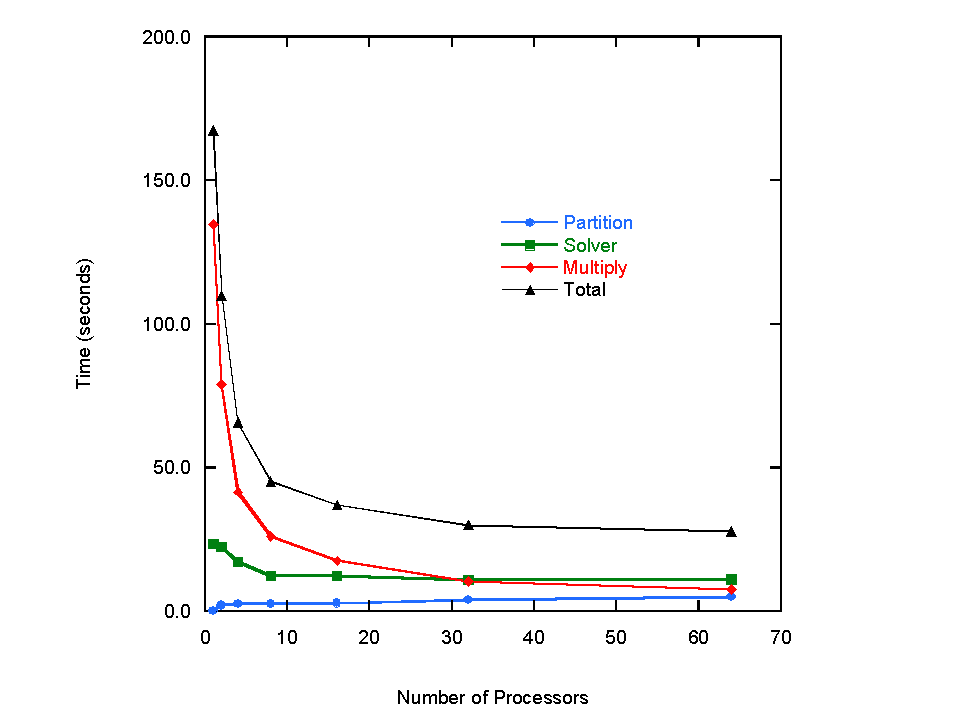
\includegraphics[width=3.5in,keepaspectratio=true]{./Fig9}
\caption{\label{ds} Strong scaling results for a dynamic simulation calculation
using on the WECC network}
\end{figure}
The algorithm has a dense matrix solve at the start and then a sequence of matrix
transpose-vector multiplies in the integration loop. The initial dense linear
solve is moderately scalable (up to about 8 processors)
and the transpose-multiply more so. The partitioner
is not scaling but only begins to contribute significantly to the overall
performance at large core counts. Overall, reasonable scaling is seen out to 32
processors but there is still a slight decrease all the way to 64 processors.

Overall, reasonable levels of scaling are seen for the powerflow and
dynamic simulation applications. However, the relatively
small size of today's power grid problems makes it difficult to achieve high
levels of scalability.  Beyond conventional scaling to larger size problems,
the power grid industry is also interested in using
computation in the context of real-time control to make operational decisions
about running the electric power grid. This requires reducing
the overall time to solution for fixed sized problems. Again, there are many
challenges. Most conventional HPC applications have relatively short setup
phases and extended computational phases that can be used to amortize the cost
of distributing and initializing the calculation. This is not the case for many
power grid applications and the cost of input, setup, initialization and output
can be a major fraction of the total run time. Thus, reducing overall
computational time requires reduction in all phases of the computation, instead
of focusing on only a few parts of it. These problems tend to cluster around the
areas of input and output and are aggravated by the relatively unstructured
nature of the data. Mapping the data associated with particular buses and
branches to the actual objects corresponding to those buses and branches tends
to be a complicated exercise in distributed hashing that is both complicated in
itself and a source of communication overhead.

\section{Conclusions}
This paper has described a framework for creating power grid applications that
run on HPC platforms. Most of the parallel programming has been embedded in high
level abstractions and the application developer is left to write the portions
of the code that express the actual detailed models and the equations that describe
them. Almost all the parallization has been buried inside the
framework components. The GridPACK\texttrademark framework has, to date, been
used to develop a number of power grid applications, These include powerflow,
dynamic simulation, and contingency analysis based on both powerflow and dynamic
simulation calculations. A state estimation application is currently in
development and applications based on Kalman filter analysis and optimization
are planned in the next year. The existing applications have demonstrated that
GridPACK has the flexibility to implement a range of calculations using a
relatively small number of modules with reasonable levels of scalability. As the
scale of power grid applications increases, we anticipate that the performance
gains from using parallel computing will increase as well.

GridPACK\texttrademark is distributed under a BSD open-source license and is
available for download at https://gridpack.org.

\section{Acknowledgments}
We wish to thank Mahantesh Halappanavar for the visualization of the WECC
partition in Figure \ref{wecc}.
Funding for this work was provided by the U.S. Department of Energy's Office of
Electricity through its Advanced Grid Modeling Program.
Additional funding was provided by the Future Power Grid Initiative at Pacific
Northwest National Laboratory through the Laboratory Directed Research and
Development program.
Pacific Northwest National Laboratory is located in Richland, WA and is operated
by Battelle Memorial Institute under contract DE-AC05-76RLO1830 with the U.S.
Department of Energy.

\bibliographystyle{abbrv}
\bibliography{gridpack}
\end{document}
